% Generated by Sphinx.
\def\sphinxdocclass{report}
\documentclass[letterpaper,10pt,english]{sphinxmanual}
\usepackage[utf8]{inputenc}
\DeclareUnicodeCharacter{00A0}{\nobreakspace}
\usepackage{cmap}
\usepackage[T1]{fontenc}

\usepackage{babel}
\usepackage{times}
\usepackage[Bjarne]{fncychap}
\usepackage{longtable}
\usepackage{sphinx}
\usepackage{multirow}
\usepackage{eqparbox}


\addto\captionsenglish{\renewcommand{\figurename}{Fig. }}
\addto\captionsenglish{\renewcommand{\tablename}{Table }}
\SetupFloatingEnvironment{literal-block}{name=Listing }



\title{Nboat Documentation}
\date{March 25, 2018}
\release{0.1}
\author{Davi Henrique}
\newcommand{\sphinxlogo}{}
\renewcommand{\releasename}{Release}
\setcounter{tocdepth}{2}
\makeindex

\makeatletter
\def\PYG@reset{\let\PYG@it=\relax \let\PYG@bf=\relax%
    \let\PYG@ul=\relax \let\PYG@tc=\relax%
    \let\PYG@bc=\relax \let\PYG@ff=\relax}
\def\PYG@tok#1{\csname PYG@tok@#1\endcsname}
\def\PYG@toks#1+{\ifx\relax#1\empty\else%
    \PYG@tok{#1}\expandafter\PYG@toks\fi}
\def\PYG@do#1{\PYG@bc{\PYG@tc{\PYG@ul{%
    \PYG@it{\PYG@bf{\PYG@ff{#1}}}}}}}
\def\PYG#1#2{\PYG@reset\PYG@toks#1+\relax+\PYG@do{#2}}

\expandafter\def\csname PYG@tok@gd\endcsname{\def\PYG@tc##1{\textcolor[rgb]{0.63,0.00,0.00}{##1}}}
\expandafter\def\csname PYG@tok@gu\endcsname{\let\PYG@bf=\textbf\def\PYG@tc##1{\textcolor[rgb]{0.50,0.00,0.50}{##1}}}
\expandafter\def\csname PYG@tok@gt\endcsname{\def\PYG@tc##1{\textcolor[rgb]{0.00,0.27,0.87}{##1}}}
\expandafter\def\csname PYG@tok@gs\endcsname{\let\PYG@bf=\textbf}
\expandafter\def\csname PYG@tok@gr\endcsname{\def\PYG@tc##1{\textcolor[rgb]{1.00,0.00,0.00}{##1}}}
\expandafter\def\csname PYG@tok@cm\endcsname{\let\PYG@it=\textit\def\PYG@tc##1{\textcolor[rgb]{0.25,0.50,0.56}{##1}}}
\expandafter\def\csname PYG@tok@vg\endcsname{\def\PYG@tc##1{\textcolor[rgb]{0.73,0.38,0.84}{##1}}}
\expandafter\def\csname PYG@tok@vi\endcsname{\def\PYG@tc##1{\textcolor[rgb]{0.73,0.38,0.84}{##1}}}
\expandafter\def\csname PYG@tok@mh\endcsname{\def\PYG@tc##1{\textcolor[rgb]{0.13,0.50,0.31}{##1}}}
\expandafter\def\csname PYG@tok@cs\endcsname{\def\PYG@tc##1{\textcolor[rgb]{0.25,0.50,0.56}{##1}}\def\PYG@bc##1{\setlength{\fboxsep}{0pt}\colorbox[rgb]{1.00,0.94,0.94}{\strut ##1}}}
\expandafter\def\csname PYG@tok@ge\endcsname{\let\PYG@it=\textit}
\expandafter\def\csname PYG@tok@vc\endcsname{\def\PYG@tc##1{\textcolor[rgb]{0.73,0.38,0.84}{##1}}}
\expandafter\def\csname PYG@tok@il\endcsname{\def\PYG@tc##1{\textcolor[rgb]{0.13,0.50,0.31}{##1}}}
\expandafter\def\csname PYG@tok@go\endcsname{\def\PYG@tc##1{\textcolor[rgb]{0.20,0.20,0.20}{##1}}}
\expandafter\def\csname PYG@tok@cp\endcsname{\def\PYG@tc##1{\textcolor[rgb]{0.00,0.44,0.13}{##1}}}
\expandafter\def\csname PYG@tok@gi\endcsname{\def\PYG@tc##1{\textcolor[rgb]{0.00,0.63,0.00}{##1}}}
\expandafter\def\csname PYG@tok@gh\endcsname{\let\PYG@bf=\textbf\def\PYG@tc##1{\textcolor[rgb]{0.00,0.00,0.50}{##1}}}
\expandafter\def\csname PYG@tok@ni\endcsname{\let\PYG@bf=\textbf\def\PYG@tc##1{\textcolor[rgb]{0.84,0.33,0.22}{##1}}}
\expandafter\def\csname PYG@tok@nl\endcsname{\let\PYG@bf=\textbf\def\PYG@tc##1{\textcolor[rgb]{0.00,0.13,0.44}{##1}}}
\expandafter\def\csname PYG@tok@nn\endcsname{\let\PYG@bf=\textbf\def\PYG@tc##1{\textcolor[rgb]{0.05,0.52,0.71}{##1}}}
\expandafter\def\csname PYG@tok@no\endcsname{\def\PYG@tc##1{\textcolor[rgb]{0.38,0.68,0.84}{##1}}}
\expandafter\def\csname PYG@tok@na\endcsname{\def\PYG@tc##1{\textcolor[rgb]{0.25,0.44,0.63}{##1}}}
\expandafter\def\csname PYG@tok@nb\endcsname{\def\PYG@tc##1{\textcolor[rgb]{0.00,0.44,0.13}{##1}}}
\expandafter\def\csname PYG@tok@nc\endcsname{\let\PYG@bf=\textbf\def\PYG@tc##1{\textcolor[rgb]{0.05,0.52,0.71}{##1}}}
\expandafter\def\csname PYG@tok@nd\endcsname{\let\PYG@bf=\textbf\def\PYG@tc##1{\textcolor[rgb]{0.33,0.33,0.33}{##1}}}
\expandafter\def\csname PYG@tok@ne\endcsname{\def\PYG@tc##1{\textcolor[rgb]{0.00,0.44,0.13}{##1}}}
\expandafter\def\csname PYG@tok@nf\endcsname{\def\PYG@tc##1{\textcolor[rgb]{0.02,0.16,0.49}{##1}}}
\expandafter\def\csname PYG@tok@si\endcsname{\let\PYG@it=\textit\def\PYG@tc##1{\textcolor[rgb]{0.44,0.63,0.82}{##1}}}
\expandafter\def\csname PYG@tok@s2\endcsname{\def\PYG@tc##1{\textcolor[rgb]{0.25,0.44,0.63}{##1}}}
\expandafter\def\csname PYG@tok@nt\endcsname{\let\PYG@bf=\textbf\def\PYG@tc##1{\textcolor[rgb]{0.02,0.16,0.45}{##1}}}
\expandafter\def\csname PYG@tok@nv\endcsname{\def\PYG@tc##1{\textcolor[rgb]{0.73,0.38,0.84}{##1}}}
\expandafter\def\csname PYG@tok@s1\endcsname{\def\PYG@tc##1{\textcolor[rgb]{0.25,0.44,0.63}{##1}}}
\expandafter\def\csname PYG@tok@ch\endcsname{\let\PYG@it=\textit\def\PYG@tc##1{\textcolor[rgb]{0.25,0.50,0.56}{##1}}}
\expandafter\def\csname PYG@tok@m\endcsname{\def\PYG@tc##1{\textcolor[rgb]{0.13,0.50,0.31}{##1}}}
\expandafter\def\csname PYG@tok@gp\endcsname{\let\PYG@bf=\textbf\def\PYG@tc##1{\textcolor[rgb]{0.78,0.36,0.04}{##1}}}
\expandafter\def\csname PYG@tok@sh\endcsname{\def\PYG@tc##1{\textcolor[rgb]{0.25,0.44,0.63}{##1}}}
\expandafter\def\csname PYG@tok@ow\endcsname{\let\PYG@bf=\textbf\def\PYG@tc##1{\textcolor[rgb]{0.00,0.44,0.13}{##1}}}
\expandafter\def\csname PYG@tok@sx\endcsname{\def\PYG@tc##1{\textcolor[rgb]{0.78,0.36,0.04}{##1}}}
\expandafter\def\csname PYG@tok@bp\endcsname{\def\PYG@tc##1{\textcolor[rgb]{0.00,0.44,0.13}{##1}}}
\expandafter\def\csname PYG@tok@c1\endcsname{\let\PYG@it=\textit\def\PYG@tc##1{\textcolor[rgb]{0.25,0.50,0.56}{##1}}}
\expandafter\def\csname PYG@tok@o\endcsname{\def\PYG@tc##1{\textcolor[rgb]{0.40,0.40,0.40}{##1}}}
\expandafter\def\csname PYG@tok@kc\endcsname{\let\PYG@bf=\textbf\def\PYG@tc##1{\textcolor[rgb]{0.00,0.44,0.13}{##1}}}
\expandafter\def\csname PYG@tok@c\endcsname{\let\PYG@it=\textit\def\PYG@tc##1{\textcolor[rgb]{0.25,0.50,0.56}{##1}}}
\expandafter\def\csname PYG@tok@mf\endcsname{\def\PYG@tc##1{\textcolor[rgb]{0.13,0.50,0.31}{##1}}}
\expandafter\def\csname PYG@tok@err\endcsname{\def\PYG@bc##1{\setlength{\fboxsep}{0pt}\fcolorbox[rgb]{1.00,0.00,0.00}{1,1,1}{\strut ##1}}}
\expandafter\def\csname PYG@tok@mb\endcsname{\def\PYG@tc##1{\textcolor[rgb]{0.13,0.50,0.31}{##1}}}
\expandafter\def\csname PYG@tok@ss\endcsname{\def\PYG@tc##1{\textcolor[rgb]{0.32,0.47,0.09}{##1}}}
\expandafter\def\csname PYG@tok@sr\endcsname{\def\PYG@tc##1{\textcolor[rgb]{0.14,0.33,0.53}{##1}}}
\expandafter\def\csname PYG@tok@mo\endcsname{\def\PYG@tc##1{\textcolor[rgb]{0.13,0.50,0.31}{##1}}}
\expandafter\def\csname PYG@tok@kd\endcsname{\let\PYG@bf=\textbf\def\PYG@tc##1{\textcolor[rgb]{0.00,0.44,0.13}{##1}}}
\expandafter\def\csname PYG@tok@mi\endcsname{\def\PYG@tc##1{\textcolor[rgb]{0.13,0.50,0.31}{##1}}}
\expandafter\def\csname PYG@tok@kn\endcsname{\let\PYG@bf=\textbf\def\PYG@tc##1{\textcolor[rgb]{0.00,0.44,0.13}{##1}}}
\expandafter\def\csname PYG@tok@cpf\endcsname{\let\PYG@it=\textit\def\PYG@tc##1{\textcolor[rgb]{0.25,0.50,0.56}{##1}}}
\expandafter\def\csname PYG@tok@kr\endcsname{\let\PYG@bf=\textbf\def\PYG@tc##1{\textcolor[rgb]{0.00,0.44,0.13}{##1}}}
\expandafter\def\csname PYG@tok@s\endcsname{\def\PYG@tc##1{\textcolor[rgb]{0.25,0.44,0.63}{##1}}}
\expandafter\def\csname PYG@tok@kp\endcsname{\def\PYG@tc##1{\textcolor[rgb]{0.00,0.44,0.13}{##1}}}
\expandafter\def\csname PYG@tok@w\endcsname{\def\PYG@tc##1{\textcolor[rgb]{0.73,0.73,0.73}{##1}}}
\expandafter\def\csname PYG@tok@kt\endcsname{\def\PYG@tc##1{\textcolor[rgb]{0.56,0.13,0.00}{##1}}}
\expandafter\def\csname PYG@tok@sc\endcsname{\def\PYG@tc##1{\textcolor[rgb]{0.25,0.44,0.63}{##1}}}
\expandafter\def\csname PYG@tok@sb\endcsname{\def\PYG@tc##1{\textcolor[rgb]{0.25,0.44,0.63}{##1}}}
\expandafter\def\csname PYG@tok@k\endcsname{\let\PYG@bf=\textbf\def\PYG@tc##1{\textcolor[rgb]{0.00,0.44,0.13}{##1}}}
\expandafter\def\csname PYG@tok@se\endcsname{\let\PYG@bf=\textbf\def\PYG@tc##1{\textcolor[rgb]{0.25,0.44,0.63}{##1}}}
\expandafter\def\csname PYG@tok@sd\endcsname{\let\PYG@it=\textit\def\PYG@tc##1{\textcolor[rgb]{0.25,0.44,0.63}{##1}}}

\def\PYGZbs{\char`\\}
\def\PYGZus{\char`\_}
\def\PYGZob{\char`\{}
\def\PYGZcb{\char`\}}
\def\PYGZca{\char`\^}
\def\PYGZam{\char`\&}
\def\PYGZlt{\char`\<}
\def\PYGZgt{\char`\>}
\def\PYGZsh{\char`\#}
\def\PYGZpc{\char`\%}
\def\PYGZdl{\char`\$}
\def\PYGZhy{\char`\-}
\def\PYGZsq{\char`\'}
\def\PYGZdq{\char`\"}
\def\PYGZti{\char`\~}
% for compatibility with earlier versions
\def\PYGZat{@}
\def\PYGZlb{[}
\def\PYGZrb{]}
\makeatother

\renewcommand\PYGZsq{\textquotesingle}

\begin{document}

\maketitle
\tableofcontents
\phantomsection\label{index::doc}



\chapter{About the Boats}
\label{index:about-the-boats}\label{index:welcome-to-unmanned-surface-vehicle-simulation-for-gazebo}
{\hspace*{\fill}\includegraphics{{boats}.png}\hspace*{\fill}}

talk a little bit about the boats and the purpose of this document.

show some youtube videos of the boats in action.


\chapter{Autonomous Systems Laboratoty - PUCRS}
\label{index:autonomous-systems-laboratoty-pucrs}
talk about LSA, link to the webpage


\chapter{Summary}
\label{index:summary}

\section{Getting Started}
\label{source/getting_started/index:getting-started}\label{source/getting_started/index::doc}

\subsection{Depedencies}
\label{source/getting_started/index:depedencies}
describe OS depedendies, Gazebo, other ROS packages, other OS packages


\subsection{Compilation}
\label{source/getting_started/index:compilation}
describe how to compile the simulator


\subsection{Testing}
\label{source/getting_started/index:testing}
describe how to launch an example scenario


\section{Environmental Disturbances}
\label{source/disturbances/index:environmental-disturbances}\label{source/disturbances/index:env-disturbs}\label{source/disturbances/index::doc}
Describe how the disturbances work. describe water current and wind modules. decribe the buoyance.

Figures: show the environment, the water speed view, and the wind speed view

{\hspace*{\fill}\includegraphics{{source/disturbances/./images/env}.png}\hspace*{\fill}}

{\hspace*{\fill}\includegraphics{{source/disturbances/./images/water}.png}\hspace*{\fill}}

{\hspace*{\fill}\includegraphics{{source/disturbances/./images/wind}.png}\hspace*{\fill}}

{\hspace*{\fill}\includegraphics{{source/disturbances/./images/buoyance}.png}\hspace*{\fill}}

\begin{notice}{warning}{Warning:}
@ To be done by Marcelo
\end{notice}


\section{Supported Boats}
\label{source/boats/index:boats}\label{source/boats/index:supported-boats}\label{source/boats/index::doc}
Describe the available boats and how they were built.

Figures: show each boat

{\hspace*{\fill}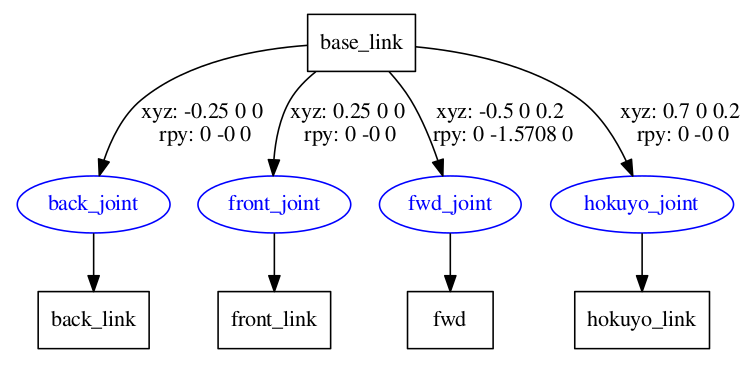
\includegraphics{{source/boats/./images/airboat}.png}\hspace*{\fill}}

{\hspace*{\fill}\includegraphics{{source/boats/./images/rudder}.png}\hspace*{\fill}}

{\hspace*{\fill}\includegraphics{{source/boats/./images/diff}.png}\hspace*{\fill}}

{\hspace*{\fill}\includegraphics{{source/boats/./images/sailing}.png}\hspace*{\fill}}

{\hspace*{\fill}\includegraphics{{source/boats/./images/wam}.png}\hspace*{\fill}}

\begin{notice}{warning}{Warning:}
@ To be done by Marcelo
\end{notice}


\section{Evaluation Scenarios}
\label{source/scenarios/index:scenarios}\label{source/scenarios/index:evaluation-scenarios}\label{source/scenarios/index::doc}
Scenarios are variations of a environment which were built to evaluate the boats performance.
List the existing evaluation scenarios.

Figures: show the scenarios

{\hspace*{\fill}\includegraphics{{source/scenarios/./images/straight}.png}\hspace*{\fill}}

{\hspace*{\fill}\includegraphics{{source/scenarios/./images/zigzag}.png}\hspace*{\fill}}

{\hspace*{\fill}\includegraphics{{source/scenarios/./images/circular}.png}\hspace*{\fill}}

\begin{notice}{warning}{Warning:}
@ To be done by Marcelo
\end{notice}


\section{Environments}
\label{source/environments/index::doc}\label{source/environments/index:environments}\label{source/environments/index:id1}
An environment describes a complete simulation scene. Cite the available environments.

Figures: show the Porto Alegre environmet

{\hspace*{\fill}\includegraphics{{source/environments/./images/poa}.png}\hspace*{\fill}}

{\hspace*{\fill}\includegraphics{{source/environments/./images/diluvio}.png}\hspace*{\fill}}

\begin{notice}{warning}{Warning:}
@ To be done by Marcelo
\end{notice}


\section{Control Strategies}
\label{source/control/index:control}\label{source/control/index:control-strategies}\label{source/control/index::doc}
The robots of this simulator have a build in movement control that we use to test some scenarios. The main objetive of this control strategy is to take the vehicle from point A to point B, point A beeing the curent position and point B beeing the desired or target position. The curent control strategy implemented is one of the simplest control strategies, called heading control.

This heading control strategy consists of doing consecutives correction of the robots heading by chosing appropriated actuators position/velocity. The idea of this control is as follows: if at each step the robot is pointing to the target point and if theres some forward velocity (in the robots frame) then eventually the vehicle will reach the desired position. Thus, what the controller does is recieve the information necessary to ajust the robots heading, namelly the curent and desired position, then calculates the proper position of the actuator to reduce the error generated by subtracting the curent and desired heading. Another part of the control must be resposible for activating the thrusters power (or at least the actuator responsable for propulsion) accordingly. The behavior generated by only using this raw erro to ajust the heading is pretty slow. To reduce this problem and set a desired behavior we use a PI strategy on the error.

The control strategy describe above is currently running in all platforms. We chose this strategy due to its simplicity that makes it quick and easy to implement. The main difference among the implemented control strategies on the platforms is how the actuation is done. For example, in the airboat the robots heading is changed according to the orientation of the fan. The rudder boat and sailboat use the rudder to change its heading. The differential boat set different thurster power on the left and right thruster to achieve heading change. The details of each control are shown below.

All of the controllers bellow use the same strategy to find the heading to be followed (preprossessing). First the it gets information about odometry (curent position) the the target position and it uses these information to find the heading to be followed. Then finds the error between the curent heading and the desired heading and uses the sign and absolute value of this error (with the PI gain) to find the apropriate action to correct it and bring the platform to the desired heading. For each platform:

\textbf{Heading control of the airboat}: Uses the heading error to find suitable fan orientation. Publishes the fan angle to /airboat/jointSetpoint.

\textbf{Forward propulsion control of the airboat}: We implemented this behavior as a set of conditions. If the distance to target is greater than 10 meters the propulsion (fan power) is 100\%. If the distance is between 2 and 10 meters then the propusion is 50\%. If the distance is less than 2 meters then the propusion is set to 0\%.

\textbf{Heading control of the boat rudder and sailboat}: These platforms use the same rudder control, wich consists of using the heading error to find suitable rudder angles. The rudder angle is published in /boat\_rudder/jointSetpoint for the boat rudder and /sailboat/jointSetpoint for the saiboat.

\textbf{Forward propulsion control of the Boat Rudder}: Similar to the Airboat.

\textbf{Forward propulsion control of the Sailboat}: Ajusts the sail position according to the wind direction.Open and closes the sail according to the wind direction on the sailboats frame: head to wind (in irons) -\textgreater{} close sail (0 degrees). rear to wind (running) -\textgreater{} open sail (90 degrees). wind betweens these positions -\textgreater{} sail position chosen linearly between 0 and 90 degrees.

\textbf{Heading control of the Differential Boat}: Uses the heading error to find suitable velocities for both thrusters (left and right). The diferential boat rotates acording to the power of both thrusters. So, for example, to rotate clockwise (on its axis) a diferential boat must use oposite power values on each thruster, for example, 10\% on the right and -10\% on the left thurster. So the controller check the error sign, chose a suitable direction of rotation and, acording to the error absolute value, chose the thuster velocity.  For example, a positive error means that the platform must rotate clockwise to reach the desired heading and a negative error means the platform must rotate counter clockwise (these relations depends of the defined frames).

\textbf{Forward propulsion control of the Differential Boat}: Uses a set of condition to decide if the boat should go forward. Use a similar set of condition describe on the Airboat forward control. To get forward velocity in the Diferential Boat it must set the same power in both thrusters.

\begin{tabulary}{\linewidth}{|L|L|}
\hline
\textsf{\relax 
Heading Control
} & \textsf{\relax 
File
}\\
\hline
Airboat
 & 
usv\_sim\_lsa/src/usv\_base\_ctrl/scripts/airboat\_control\_heading.py
\\
\hline
Differential Boat
 & 
usv\_sim\_lsa/src/usv\_base\_ctrl/scripts/diff\_control\_heading.py
\\
\hline
Rudder Boat
 & 
usv\_sim\_lsa/src/usv\_base\_ctrl/scripts/rudder\_control\_heading.py
\\
\hline
Sailboat
 & 
usv\_sim\_lsa/src/usv\_base\_ctrl/scripts/sailboat\_control\_heading.py
\\
\hline\end{tabulary}


The videos below show the control strategies described above woking at different levels of disturbance (water curent and wind).


\section{Contributors}
\label{source/contributors/index::doc}\label{source/contributors/index:contributors}
The list of contributors to this document.
\begin{itemize}
\item {} 
\href{https://amamory.github.io/}{@Alexandre Amory}

\item {} 
@Davi Henrique

\item {} 
@Luiz Marcos Gonçalves

\item {} 
@Marcelo Paravisi

\item {} 
@Vitor Jorge

\end{itemize}


\chapter{Disclaimer}
\label{index:disclaimer}
The purpose of this document is for the use of LSA group only, but we open it in case it can be usefull for someone else.
Everything you find here is without absolutly no waranty and I'm not responsible for any inconveniences or issues that might occurs.


\chapter{Feedback}
\label{index:feedback}
Don't hesitate to ask about some additional info or next guides and also if you find some mistakes, please let me know.
This can be done by submitting an issue or a push request on github.



\renewcommand{\indexname}{Index}
\printindex
\end{document}
